\documentclass[aspectratio=169,11pt]{beamer}

\usetheme{Madrid}
\usecolortheme{seahorse}
\usepackage[T1]{fontenc}
\usepackage[utf8]{inputenc}
\usepackage[polish]{babel}
\usepackage{amsmath,amssymb}
\usepackage{graphicx}
\usepackage{booktabs}
\usepackage{siunitx}
\sisetup{locale=DE}

\title{Synteza jądrowa}
\subtitle{Od gwiazd do przyszłych elektrowni}
\author{Prezentacja popularnonaukowa}
\institute{Fizyka energii}
\date{\today}

\begin{document}

\begin{frame}
  \titlepage
\end{frame}

\begin{frame}
  \frametitle{Plan prezentacji}
  \tableofcontents
\end{frame}

\section{Podstawy fizyczne}
\begin{frame}
  \frametitle{Czym jest synteza jądrowa?}
  \begin{block}{Idea}
    Lekkie jądra łączą się w cięższe. Ubytek masy układu uwalnia energię:
    \[
      E=\Delta m\,c^2.
    \]
  \end{block}
  \begin{columns}[T,onlytextwidth]
    \column{0.56\textwidth}
      \begin{itemize}
        \item Reakcja zachodzi naturalnie we wnętrzach gwiazd.
        \item Na Ziemi najłatwiej badać reakcję deuter--tryt (D--T).
        \item Produkty reakcji niosą energię kinetyczną.
      \end{itemize}
    \column{0.40\textwidth}
      \begin{exampleblock}{Reakcja D--T}
        \[
          {}^2\mathrm{H}+{}^3\mathrm{H}
          \rightarrow {}^4\mathrm{He}+n+17{,}6~\mathrm{MeV}
        \]
      \end{exampleblock}
  \end{columns}
\end{frame}

\begin{frame}
  \frametitle{Dlaczego potrzebna jest bardzo wysoka temperatura?}
  \begin{columns}[T,onlytextwidth]
    \column{0.48\textwidth}
      \begin{block}{Bariera kulombowska}
        Jądra mają dodatni ładunek i odpychają się elektrostatycznie.
        Wysoka temperatura zwiększa prawdopodobieństwo zbliżenia jąder,
        a tunelowanie kwantowe również ułatwia reakcję.
      \end{block}
      \[
        k_{\mathrm B}T \sim \text{energia ruchu cząstek}
      \]
    \column{0.48\textwidth}
      \begin{alertblock}{Ważne rozróżnienie}
        Temperatura plazmy w eksperymentach jest rzędu
        \(10^8\,\mathrm K\). To nie oznacza, że cały reaktor musi być
        równie gorący: plazmę izoluje się od ścian.
      \end{alertblock}
  \end{columns}
\end{frame}

\section{Jak utrzymać plazmę?}
\begin{frame}
  \frametitle{Plazma i kryterium Lawsona}
  \begin{block}{Plazma}
    Zjonizowany gaz złożony z elektronów i jonów. Jego zachowanie
    opisują elektromagnetyzm, mechanika płynów i fizyka kinetyczna.
  \end{block}
  Dla reakcji D--T warunek uzyskania bilansu energetycznego często
  wyraża się potrójnym iloczynem:
  \[
    nT\tau_E,
  \]
  gdzie \(n\) to gęstość paliwa, \(T\) -- temperatura, a \(\tau_E\) --
  czas utrzymania energii.
  \begin{itemize}
    \item Zwiększenie jednego czynnika może częściowo kompensować mniejszą
      wartość pozostałych.
    \item Liczy się bilans całego układu, nie tylko energia samej plazmy.
  \end{itemize}
\end{frame}

\begin{frame}
  \frametitle{Uwięzienie magnetyczne: tokamak}
  \begin{columns}[T,onlytextwidth]
    \column{0.51\textwidth}
      \begin{itemize}
        \item Silne pola magnetyczne ograniczają ruch naładowanych cząstek.
        \item Pole toroidalne i poloidalne tworzą skręcone linie pola.
        \item Prąd w plazmie pomaga wytworzyć składową poloidalną.
      \end{itemize}
      \begin{alertblock}{Wyzwanie}
        Utrzymanie stabilnej plazmy i ograniczenie jej kontaktu ze ścianą.
      \end{alertblock}
    \column{0.46\textwidth}
      \centering
      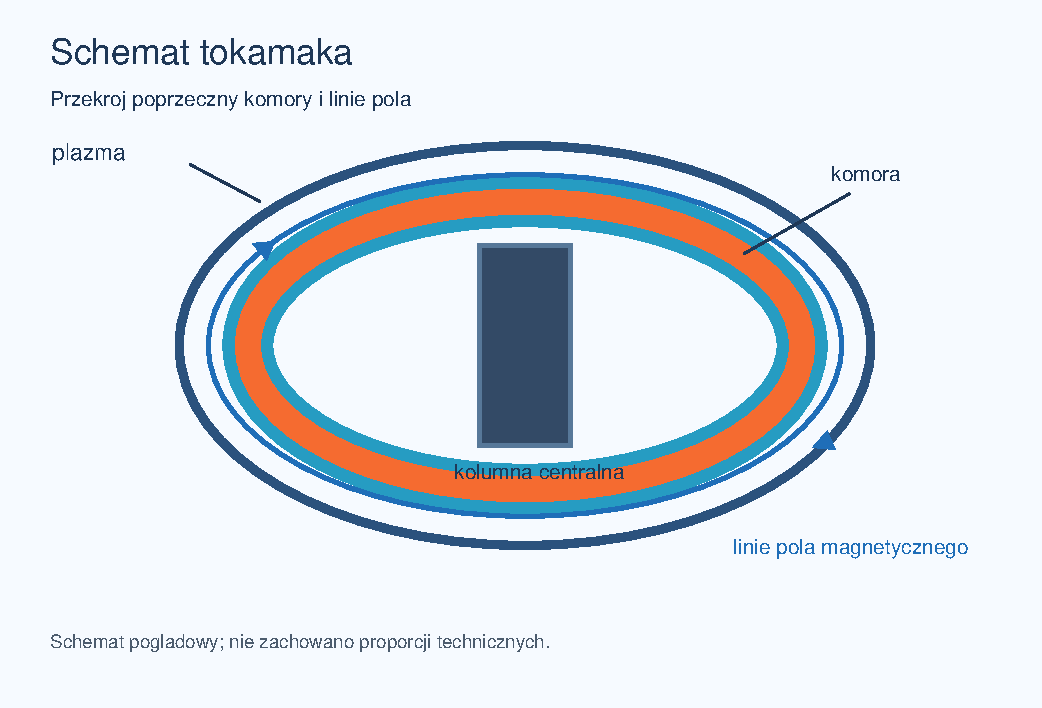
\includegraphics[width=\linewidth]{tokamak.pdf}
      {\scriptsize Schematyczny przekrój torusa tokamaka; ilustracja własna.}
  \end{columns}
\end{frame}

\begin{frame}
  \frametitle{Uwięzienie inercyjne}
  \begin{exampleblock}{Inna droga do fuzji}
    Mała kapsułka paliwa jest gwałtownie ściskana i ogrzewana krótkim
    impulsem laserowym. Reakcja zachodzi, zanim paliwo zdąży się rozprężyć.
  \end{exampleblock}
  \begin{enumerate}
    \item Energia impulsu trafia w zewnętrzną warstwę kapsułki.
    \item Ablacja tej warstwy wywołuje reakcję odrzutu i kompresję paliwa.
    \item W gorącym, gęstym obszarze mogą zajść reakcje syntezy.
  \end{enumerate}
  \begin{alertblock}{Ograniczenie}
    Powtarzalna praca elektrowni wymagałaby szybkiego, precyzyjnego
    podawania i zapłonu wielu kapsułek.
  \end{alertblock}
\end{frame}

\section{Energia i technologia}
\begin{frame}
  \frametitle{Zysk energetyczny: co właściwie mierzymy?}
  \begin{block}{Współczynnik \(Q\)}
    Dla plazmy definiuje się zwykle
    \[
      Q_{\mathrm{plasma}}=
      \frac{P_{\mathrm{fusion}}}{P_{\mathrm{heating}}},
    \]
    czyli moc syntezy podzieloną przez moc dostarczaną do ogrzewania plazmy.
  \end{block}
  \begin{itemize}
    \item \(Q_{\mathrm{plasma}}>1\) nie oznacza jeszcze dodatniego bilansu
      całej instalacji.
    \item Trzeba uwzględnić m.in. sprawność ogrzewania, magnesów,
      chłodzenia i zamiany ciepła na elektryczność.
  \end{itemize}
  \begin{alertblock}{Uwaga}
    Wynik dla plazmy i bilans energii elektrycznej całego obiektu to różne
    wielkości.
  \end{alertblock}
\end{frame}

\begin{frame}
  \frametitle{Co musi rozwiązać elektrownia fuzyjna?}
  \begin{columns}[T,onlytextwidth]
    \column{0.49\textwidth}
      \begin{block}{Fizyka i materiały}
        \begin{itemize}
          \item stabilna praca plazmy,
          \item odporność materiałów na neutrony,
          \item odprowadzanie ciepła z dywertora.
        \end{itemize}
      \end{block}
    \column{0.49\textwidth}
      \begin{block}{Paliwo i instalacja}
        \begin{itemize}
          \item produkcja trytu z litu,
          \item zdalna konserwacja elementów aktywowanych,
          \item niezawodność i konkurencyjny koszt energii.
        \end{itemize}
      \end{block}
  \end{columns}
  \[
    n+{}^6\mathrm{Li}\rightarrow{}^4\mathrm{He}+{}^3\mathrm{H}
    +4{,}8~\mathrm{MeV}
  \]
\end{frame}

\section{Podsumowanie}
\begin{frame}
  \frametitle{Najważniejsze wnioski}
  \begin{itemize}
    \item Synteza łączy lekkie jądra i uwalnia energię dzięki ubytkowi masy.
    \item Kluczowe są jednocześnie temperatura, gęstość i czas utrzymania
      plazmy.
    \item Tokamaki i uwięzienie inercyjne realizują różne strategie.
    \item Zysk plazmy nie jest tym samym co zysk energetyczny elektrowni.
  \end{itemize}
  \begin{block}{Pytanie na koniec}
    Jak przejść od udanej reakcji fuzyjnej do niezawodnego źródła energii
    elektrycznej?
  \end{block}
  \begin{exampleblock}{Kolejne etapy}
    Długotrwała praca plazmy \(\rightarrow\) test materiałów i hodowli trytu
    \(\rightarrow\) integracja reaktora \(\rightarrow\) opłacalna elektrownia.
  \end{exampleblock}
  {\footnotesize
  Wybrane źródła: ITER, \emph{What is Fusion?}; IAEA,
  \emph{Fusion Energy}; NIF, materiały o zapłonie fuzyjnym.}
\end{frame}

\end{document}
